\documentclass{report}

\usepackage{times}
\usepackage{helvet}
\usepackage{courier}
\usepackage{comment}
\usepackage{subfig}
\usepackage{relsize}
\usepackage{mathtools}
\usepackage{amsmath}
\usepackage{enumitem}
\usepackage[dvipdfmx]{graphicx}
\usepackage{adjustbox}
\usepackage{rotating}
\usepackage{multirow}
\usepackage{amssymb}
\usepackage{url}
\usepackage{listings}
\usepackage{lstlang0}

\usepackage{tikz} % Drawing sliding-tile

\usepackage[ruled,boxed,linesnumbered,noend]{algorithm2e}
\SetKwInOut{Input}{Input}
\SetKwInOut{Output}{Output}
\SetKwInOut{Side}{Side effect}
\SetKwComment{Comment}{$\triangleright$\ }{}

\setcounter{secnumdepth}{2}
%\frenchspacing

\newtheorem{definition}{Definition}

%\newcommand{\citeauthor[1]}{\cite{#1}}

\title{ヒューリスティック探索}

\author{陣内 佑 \\
東京大学 総合文化研究科}



\begin{document}

\maketitle

\tableofcontents
\newpage

\section*{まえがき}
ヒューリスティック探索はグラフ探索のサブフィールドであり、解こうとしている問題の知識を探索方法に反映させることでより効率的に探索をしよう、という分野である。

ヒューリスティック探索のイントロダクションと現在どのように発展しているのかというのをまとめてみようかと思い、本文を執筆した。
以前、さる国内の高名なAI研究者がご講演で「ヒューリスティック探索は終わった技術であり、Toy Problemしか解けない」とおっしゃった。これは全くの勘違いであるが、思い返すと仕方がないことかと思われる。というのも、日本には探索分野、特にヒューリスティック探索の研究者というのは数えるほどしかいない。大御所の方々は大変忙しく、他分野、ましては自分では終わったと思っている分野の英語論文など読まないだろう。こうなると、その分野の知識は古いままで、なおのこと終わった分野だと思ってしまいがちである、と想像される。
そこで、若輩者ながら、数少ない日本語の書けるヒューリスティック探索アルゴリズムの研究者として、日本のAI研究に微力を添えようと日本語の教科書を書こうと思った次第である。


\chapter{イントロダクション}
\label{ch:introduction}

人は様々な問題を探索によって解決している。
例えば飛行機で成田からロンドンに行く安い/速い方法などを計画するのは探索の一つである。
%一昔前は探索こそが人類の知であるという価値観が広くあり、囲碁、将棋、チェスなどのゲームはそれを競う競技であるとして。
あるいは囲碁、将棋、チェスなどのゲームも、ある手を選んだ時にどのような局面につながるのかを先読みし、選ぶべき次の一手を探索する。
このような様々な問題はグラフ探索問題として統合してモデルすることが出来る。
%もちろん、それぞれの問題はそれぞれの特徴があり、それぞれで効率的な解法が異なる。


% This chapter is ...
この章ではまず、\ref{sec:state-space-problem}節ではグラフ探索手法が用いられる問題として状態空間問題を定義する。
状態空間問題は様々な応用問題を含む。
次に\ref{sec:search-problem}節でグラフ探索で解くことの出来る問題をいくつか紹介する。
経路探索問題や倉庫番問題など、応用がありつつ、かつ分かりやすい問題を選んだ。これらの問題はすべて探索研究界隈でベンチマークとして広く使われているものである。


\section{状態空間問題 (State-Space Problem)}
\label{sec:state-space-problem}
探索問題は初期状態とゴール条件が与えられたとき、ゴール条件を満たすための経路を返すのが探索問題である。
このテキストでは探索問題の主な対象として状態空間問題(State-space problem)を考える。状態空間問題$P = (S, A, s, T)$は状態の集合$S$、初期状態$s \in S$、ゴール集合$T \in S$、アクション集合$A = {a_1, ....,a_n}$、$a_i : S \rightarrow S$がある。アクションはある状態を次の状態に遷移させる関数である。
状態空間問題の解は初期状態からゴール状態へ遷移させるアクションの列を求めることである。

よって、状態空間問題はグラフにモデルすることで考えやすくなる。
状態空間グラフは以下のように定義される。

\begin{definition}[状態空間グラフ、State-space graph]
問題グラフ$G = (V, E, s, T)$は状態空間問題$P = (S, A, s, T)$に対して以下のように定義される。ノード集合 $V = S$、初期ノード$s \in S$、ゴールノード集合$T$、エッジ集合$E\subseteq V \times V$。エッジ$u,v\in E$は$a(u) = v$となる$a\in A$が存在する場合に存在し、そしてその場合にのみ存在する(iff)。
\end{definition}

状態空間問題の解は以下の定義である。

\begin{definition}[解、Solution]
解$\pi = (a_1,a_2...,a_k)$はアクション$a_i \in A$の(順序付)配列であり、初期状態$s$からゴール状態$t \in T$へ遷移させる。すなわち、$u_i \in S$,$i \in \{0,1,...,k\}$, $u_0 = s, u_k = t$が存在し、$u_i = a_i(u_{i-1})$となる。
\end{definition}

どのような解を見つけたいかは問題に依存する。どのような解でもよいのか、経路を最短にする解が良いのか、様々な問題が考えられる。
多くの問題では経路の{\bf コスト}の合計を最小にすることを目的とする。
すなわち、アクションに対して

\begin{definition}[コスト付き状態空間問題、Weighted state-space problem]
コスト付き状態空間問題$P = (S, A, s, T, w)$は状態空間問題の定義に加え、コスト関数$w: A \rightarrow \mathbb{R}$がある。経路$(a_1,...,a_k)$のコストは$\sum^k_{i=1}w(a_i)$と定義される。ある解が可能なすべての解の中でコストが最小である場合、その解を最適解(optimal cost)であると言う。
\end{definition}

コスト付き状態空間問題は重み付き(コスト付き)グラフとしてモデルすることが出来る。すなわち、$G = (V, E, s, T, w)$は状態空間グラフの定義に加え、エッジの重み$w: E \leftarrow \mathbb{R}$を持つ。

%ただし、状態空間グラフをすべて陽に変換し、すべてのノード・エッジを保持することは効率が良くないことが多い。
ただし、探索アルゴリズムは状態空間グラフのノード・エッジ全てを保持する必要はない。
全てのノード・エッジを保持した状態空間グラフを特に陽状態空間グラフ(explicit state-space graph)と呼ぶとする\footnote{他に対訳を見つけることが出来なかったため、陽・陰状態空間グラフという訳は筆者がつけた。}。このようなグラフは、例えば隣接行列を用いて表すことが出来る。隣接行列$M$は行と列の大きさが$|V|$である正方行列であり、エッジ$(v_i, v_j)$が存在するならば$M_{i,j}=1$、なければ$M_{i,j}=0$とする行列である。
このような表現方法の問題点は行列の大きさが$|V|^2$であるため、大きな状態空間を保持することが出来ないことである。
例えば、\index{sec:search-problem}節で紹介する15-puzzleは状態の数が$|V|=15!/2$であるため、隣接行列を保持することは現在のコンピュータでは非常に困難である。

そこで、探索アルゴリズムは多くの場合初期ノードとノード展開関数による陰状態空間グラフで表せられる。

\begin{definition}[陰状態空間グラフ、Implicit state-space graph]
陰状態空間グラフは初期状態$s \in V$、ゴール条件Goal: $V \rightarrow B = \{false, true\}$、ノード展開関数Expand: $V \rightarrow 2^V$によって与えられる。
\end{definition}

探索の開始時、エージェントは初期ノードのみを保持する。エージェントは保持しているノードに対してExpandを適用することによって、新しいノードとエッジをグラフに加える。これを求める解を見つけるまで繰り返す。

%\begin{example}

%\end{example}

これによって、エージェントは解を見つけるまでのノード・エッジだけ保持して必要な解を見つけることが出来る。
大まかには、情報なし探索による陰グラフは陽グラフよりも指数的に小さく、ヒューリスティック探索による陰グラフは情報なし探索による陰グラフよりも更に指数的に小さいことが多い。


\section{探索問題の例}
\label{sec:search-problem}

グラフ探索によって効率的に解くことが出来ると知られているドメインをいくつか紹介する。


\subsection{グリッド経路探索 (Grid Path-finding)}

グリッド経路探索問題は2次元のグリッド上で初期配置からゴール位置までの経路を求める問題である。グリッドには障害物がおかれ、通れない箇所がある。

グリッド経路探索はゲームAIなどで問題となる。


Starcraft 1ではA*探索が使われていた。
%しかしマルチエージェント
マルチエージェント経路探索の場合はflocking / swarm AIが使われている。
Starcraft 2では


\subsection{スライディングタイル (Sliding-tile Puzzle)}

多くの一人ゲームはグラフ探索問題に帰着することが出来る。スライディングタイルはその例であり、ヒューリスティック探索研究においてメジャーなベンチマーク問題でもある (図\ref{fig:15-puzzle})\footnote{機械学習・画像処理におけるところのMNISTだろうか}。
$1$から$(n^2)-1$までの数字が振られたタイルが$n\times n$の正方形に並べられている。正方形には一つだけ{\it ブランク}と呼ばれるタイルのない位置があり、四方に隣り合うタイルのいずれかをその位置に移動する(スライドする)ことが出来る。スライディングタイル問題は、与えられた初期状態からスライドを繰り返し、ゴール状態にたどり着く経路を求める問題である。

\begin{figure}
\centering
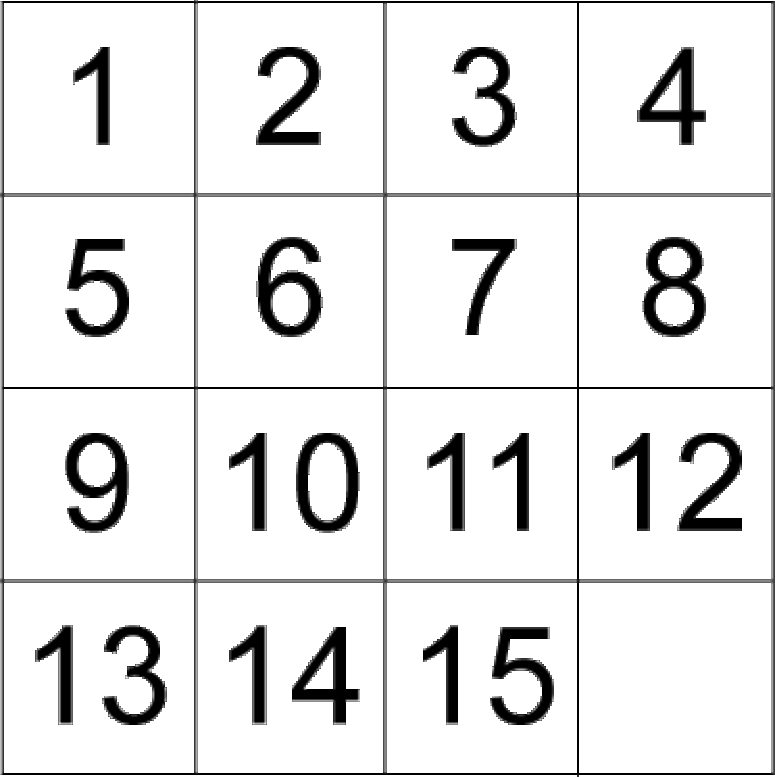
\includegraphics[width=0.4\textwidth]{figures/15-puzzle.pdf}
\caption{15パズルのゴール状態の例}
\label{fig:15-puzzle}
\end{figure}

スライディングタイルの到達可能な状態の数は$|V| = (n^2)!/2$\footnote{スライディングタイルは偶奇性があり、到達不可能な状態がある\cite{TODO}。}であり、$n$に対して指数的に増加する。
可能なアクションは$A= \{up, down, left, right\}$の4つであり、アクションにかかるコストはすべて同じとする。

後述するが、ヒューリスティック探索のためには状態からゴール状態までの距離(コスト)の下界(lower bound)を計算する必要がある。
スライディングタイルにおける下界の求め方として最もシンプルなものは{\it マンハッタン距離ヒューリスティック}である。マンハッタン距離ヒューリスティックは各タイルの現在状態の位置とゴール状態の位置のマンハッタン距離の総和を取る。可能なアクションはすべて一つしかタイルを動かさないので、一回のアクションでマンハッタン距離は最大で1しか縮まらない。よって、マンハッタン距離はゴールまでの距離の下界である。

%ちなみに、スライディングタイルはpermutation problemの一つである。

\subsection{Multiple Sequence Alignment (MSA)}

生物学・進化学では遺伝子配列・アミノ酸配列の編集距離(edit distance)を比較することでニ個体がどれだけ親しいかを推定することが広く研究されている。
MSAは複数の遺伝子・アミノ酸配列が与えられた時、それらの配列間の編集距離とその時出来上がった配列を求める問題である。
2つの配列に対してそれぞれコストの定義された編集操作を繰り返し、同一の配列に並べ替える手続きをアライメントと呼ぶ。
2つの配列の編集距離はアライメントのコストの最小値である。
3つ以上の配列における距離の定義は様々考えられるが、ここでは全ての配列のペアの編集距離の総和を用いる。

MSAにおける可能な編集操作は置換と挿入である。置換は配列のある要素(DNAかアミノ酸)を別の要素に入れ替える操作であり、挿入は配列のある位置に要素を挿入する操作である。例えば(ABC, BCB, CB)の3つの配列のアライメントを考える。図\ref{fig:msa-cost}は置換と編集に対するコストの例である。-は欠損、すなわち挿入操作が行われたことを示す。アミノ酸配列における有名なコスト表としてPAM250があるが、ここでは簡単のため仮のコスト表を用いる\cite{MSA}。
図\ref{fig:msa-solution}はこのコスト表を用いたアライメントの例である。
このとき、例えば配列ABC-と-BCBの編集距離は(A,-)、 (B,B)、 (C,C)、 (-,B)のコストの総和であるので、図\ref{fig:msa-cost}を参照し、$5+0+1+5=11$である。(-BCB, --CB)の距離は$6$, (--CB, ABC-)の距離は$16$であるので、3配列の編集距離は$11+6+16=33$である。

$n$配列のMSAは$n$次元のグリッドの経路探索問題に帰着することが出来る(図\ref{fig:msa-to-grid})。


\begin{figure}
\centering
\subfloat[MSAの解の例]{
\begin{tabular}{ccccc}
	A & B & C & - \\
	- & B & C & B \\
	- & - & C & B \\
\end{tabular}
\label{fig:msa-solution}
} \hspace{4pt}
\subfloat[操作コスト表の例]{
\begin{tabular}{c|cccc}
	  & A & B & C & - \\ \hline
	A & 0 & 1 & 2 & 5 \\
	B &   & 0 & 3 & 5 \\
	C &   &   & 1 & 5 \\
	- &   &   &   & 0 \\	
\end{tabular}
\label{fig:msa-cost}
} \hspace{4pt}
\subfloat[グリッド経路探索への帰着]{
\begin{tabular}{c|cccc}
	  &   & A & B & C \\ \hline
	  & X & X &   &   \\
	B &   &   & X &   \\
	C &   &   &   & X \\
	B &   &   &   & X \\
\end{tabular}
\label{fig:msa-to-grid}
}
\end{figure}



\subsection{倉庫番 (Sokoban)}
倉庫番(Sokoban)は日本発のパズルゲームであり、倉庫の荷物を押していくことで指定された位置に置くというゲームである。現在でも様々なゲームでゲーム内ミニゲームとして親しまれている。
プレイヤーは「荷物の後ろに回って押す」ことしか出来ず、引っ張ったり、横から動かしたりすることが出来ない。また、荷物の上を通ることも出来ない。

グラフ探索問題として倉庫番を考えるときに重要であるのは、倉庫番は{\it 不可逆な}アクション(irreversible)があることである。
グリッド経路探索やスライディングタイルは{\it 可逆な} (reversible)問題である。
全てのアクション$a \in A$に対して$a^{-1} \in A$が存在し、$a(a^{-1}(s)) = s$かつ$a^{-1}(a(s)) = s$となる場合、問題は可逆であると言う。
可逆な問題は対応するアクションのコストが同じであれば無向グラフとしてモデルすることも出来、初期状態から到達できる状態は、すべて初期状態に戻ることが出来る。
一方、不可逆な問題ではこれが保証されず、詰み(trap)状態に陥る可能性がある。

倉庫番では荷物を押すことは出来ても引っ張ることが出来ないため、不可逆な問題である。例えば、荷物を部屋の隅に置いてしまうと戻すことが出来ないため、詰み状態に陥る可能性がある問題である。
このような性質を持つ問題では特にグラフ探索による先読みが効果的である。


%倉庫の中には荷物がおかれ、エージェント(プレイヤー)は迷路を動き回り、
%このゲームで面白い/難しいのは、「荷物の後ろに回って押す」ことしか出来ず、引っ張ったり、横から動かしたりすることが出来ないという点である。

\subsection{巡回セールスパーソン問題 (Travelling Salesperson Problem)}

セールスパーソンはいくつかの都市に回って営業を行わなければならない。都市間の距離(=コスト)は事前に与えられている。
TSPは全ての都市を最短距離で回ってはじめの都市に戻る経路を求める、という問題である。

$n$個の都市があるとすると(最適・非最適含む)解の数は$(n-1)!/2$個である。
TSPはNP完全であることが知られている。
TSPの下界としては{\it 最小全域木} (minimum spanning tree)のコストがよく用いられる。
グラフの{\it 全域木} (spanning tree)は全てのノードを含むループを含まない部分グラフである。
最小全域木は全域木のうち最もエッジコストの総和が小さいものである。
未訪問の都市によるグラフの最小全域木はTSPの下界となることが知られている。




%%%%%%%%%%%%%%%%%%%%%%%%%%%%%%%%%%%%%%%%%%%%%%%%%
%%% CHAPTER: Blind Search
%%%%%%%%%%%%%%%%%%%%%%%%%%%%%%%%%%%%%%%%%%%%%%%%%
\chapter{情報なし探索 (Blind Search)}
\label{ch:blind-search}
最もシンプルなグラフ探索は問題(ドメイン)の知識を利用しない探索である。
すなわち、何も情報を見ずに探索を行うという意味でBlind Searchと言われる。
Blind searchの例としては幅優先探索・深さ優先探索などがあり、問題を選べばこれらの手法によって十二分に効率的な探索を行うことが出来る。
これらの探索手法は競技プログラミングでもよく解法として使われる(らしい)\footnote{TODO: 典拠}。また、いわゆるコーディング面接でもグラフ探索アルゴリズムは頻出である(らしい)\footnote{TODO: 典拠}。
\ref{ch:search-performance}章はグラフ探索の高速化の紹介をするので、特に競技プログラミングに興味がある場合はそちらも参照されたい。



\section{木探索アルゴリズム (Tree Search Algorithm)}
\label{sec:tree-search-algorithm}
木は
木探索はグラフに対して適用することが出来る。
図\ref{X}は木探索の例である。
陽グラフのあるノードが初期状態から複数の経路でたどり着ける場合、同じ状態を表すノードが木探索による陰グラフに複数現れるということが生じる。このようなノードを重複(duplicate)と呼ぶ。ノードの重複は計算資源を無駄にするだけなのでなんとかして避けたいものであり、重複の効率的な検出方法は探索研究の大きなヤマの一つである。
%同じ状態を複数回展開すると計算資源を無駄にすることになるのでなるべく重複を避けたい。


\begin{algorithm}
\caption{Implicit Tree Search}
\label{alg:implicit-tree-search}
	\Input{Implicit problem tree with initial node $s$, weight function $w$, successor generation function $Expand$, goal function $Goal$}
	\Output{Path from $s$ to a goal node $t \in T$, or $\emptyset$ if no such path exists}
	$Open \leftarrow \{s\}$\;
	\While{$Open \neq \emptyset$} {
		$u \leftarrow Open.pop()$\;
		\If {$Goal(u)$} {
			\Return $Path(u)$\;
		}
		$Succ(u) \leftarrow Expand(u)$\;
		\For {each $v \in Succ(u)$} {
			$Open.insert(v)$\;
			$parent(v) \leftarrow u$\;
		}
 	}
	\Return $\emptyset$\;
\end{algorithm}

\begin{enumerate}
\item 展開済みノード: $Expand(u)$によって子ノードが参照されたノードを指す。
\item 生成済みノード: $Open.insert(v)$によってOpenに一度でも入れられたノードを指す。

\end{enumerate}

木探索ベースのアルゴリズムの問題は、解が存在しない場合に停止性を満たさないことである。
よって、この手法は解が間違いなく存在することが分かっている問題に対して適用される。あるいは、解が存在することを判定してから用いる。

\section{グラフ探索アルゴリズム (Graph Search Algorithm)}
\label{sec:graph-search-algorithm}

木探索がノードの重複を無視して探索を行うのに対して、グラフ探索アルゴリズムはノードの重複を確認して探索を行う。
ノードの重複の確認にはいくつかメリットがある。一つは、停止性を満たすことである。すなわち、最悪グラフのノードをすべて展開して停止する。もう一つは、重複して同じ状態を展開せずにすむことである。


\begin{algorithm}
\caption{Implicit Graph Search}
\label{alg:implicit-graph-search}
	\Input{Implicit problem graph with initial node $s$, weight function $w$, successor generation function $Expand$, goal function $Goal$}
	\Output{Path from $s$ to a goal node $t \in T$, or $\emptyset$ if no such path exists}
	$Closed \leftarrow \emptyset$\;
	$Open \leftarrow \{s\}$\;
	\While{$Open \neq \emptyset$} {
		$u \leftarrow Open.pop()$\;
		$Closed.insert(u)$\;
		\If {$Goal(u)$} {
			\Return $Path(u)$\;
		}
		$Succ(u) \leftarrow Expand(u)$\;
		\For {each $v \in Succ(u)$} {
			$Improve(u, v)$\;
		}
 	}
	\Return $\emptyset$\;
\end{algorithm}

\begin{algorithm}
\caption{$Improve(u,v)$}
\label{alg:improve}
	\Input{Node u and its successor $v$}
	\Side{Update parent of $v$, $Open$, and $Closed$}
	\If{$v \notin Closed \cup Open$} {
		$Open.insert(v)$\;
		$parent(v) \leftarrow u$\;
	}
\end{algorithm}

\section{幅優先探索 (Breadth-First Search)}
\label{sec:breadth-first-search}

Open listはPriority queueであり、何らかの基準によってセットからpopするノードを決めている。
幅優先探索は探索の「幅」を最大化するようにノードを選択する。

初期状態から現在状態にたどり着くまでのコストをノードの$g$値と定義する。

\begin{algorithm}
\caption{Breadth-First Search: $Open.pop()$}
\label{alg:brfs-open}
	\Output{Node $u$}
	\Return $\arg \min_n g(n)$
\end{algorithm}

\section{深さ優先探索 (Depth-First Search)}
\label{sec:depth-first-search}

ゴールがある程度深い所にあり、浅い場所にはないと事前に分かっている場合に上手く行く。


\begin{algorithm}
\caption{Depth-First Search: $Open.pop()$}
\label{alg:dfs-open}
	\Output{Node $u$}
	\Return $\arg \max_n g(n)$
\end{algorithm}

%\section{ダイクストラ法}



\chapter{ヒューリスティック探索}
\label{ch:heuristic-search}

\ref{ch:blind-search}章では問題の知識を利用しないグラフ探索手法について解説した。
本章では問題の知識を利用することでより効率的なグラフ探索を行う手法、特にヒューリスティック探索について解説する。

\section{ヒューリスティックとは?}
\label{sec:heursitic}

経路探索問題を幅優先探索で解くことを考えよう。
図\ref{fig:grid}の初期状態からゴールへの最短経路の長さはXである。このとき、幅優先探索は図\ref{fig:grid-brfs}の領域を探索する。

しかし人間が経路探索を行うときにこんなに広い領域を探索しないだろう。なぜか。
それは人間が問題の特徴を利用して、このノードを探索したほうがよいだろう、という推論を働かせているからである。

問題の特徴を利用してノードの{\bf 有望さ}をヒューリスティック関数として定量化し、ヒューリスティック関数を利用した探索アルゴリズムをヒューリスティック探索と呼ぶ。

ヒューリスティック関数は人間が自分の知識を利用してコーディングする場合もあるが、特にプランニング問題などでは自動的にヒューリスティックを生成する手法も広く使われている。


\section{ヒューリスティック関数}
\label{sec:heuristic-function}

ヒューリスティック関数はある状態からゴールまでの距離の見積もりである。

\begin{definition}[ヒューリスティック関数]
ヒューリスティック関数$h$はノードの評価関数である。$h: V \rightarrow \mathbb{R}_{\geq 0}$
\end{definition}

\begin{definition}[許容的なヒューリスティック]
ヒューリスティック関数$h$は最適解のコストの下界である場合、許容的である。すなわち、全てのノード$u \in V$に対して$h(u) \leq \delta(u, T)$が成り立つ。
\end{definition}

\begin{definition}[無矛盾なヒューリスティック]
ヒューリスティック関数$h$は全てのエッジ$e = (u, v) \in E$に対して$h(u) \leq h(v) + w(u,v)$が成り立つ場合、無矛盾である。
\end{definition}


\section{A*探索}
\label{sec:astar-search}

A*探索はヒューリスティック探索の代名詞である、最もドミナントな手法である。
A*探索は以下のf値が最小となるノードを優先して探索を行う。

\begin{equation}
	f(n) = g(n) + h(n)
\end{equation}

\begin{algorithm}
\caption{A*: $Open.pop()$}
\label{alg:astar-open}
	\Output{Node $u$}
	\Return $\arg \min_n f(n)$
\end{algorithm}

Shakey the Robot
Optimality





\subsection{重み付きA*探索}
\label{sec:weighted-astar-search}

許容的なヒューリスティックを用いた場合、最適解のコスト$f^*$に対して、発見される解のコストが$w f^*$以下であることを保証する。

\begin{equation}
	f_w(n) = g(n) + w h(n)
\end{equation}

\begin{algorithm}
\caption{w A*: $Open.pop()$}
\label{alg:wastar-open}
	\Output{Node $u$}
	\Return $\arg \min_n f_w(n)$
\end{algorithm}

\section{貪欲最良優先探索 (Greedy Best-First Search)}
\label{sec:greedy-best-first-search}

解のクオリティに保証がない。

\begin{algorithm}
\caption{Greedy Best-First Search: $Open.pop()$}
\label{alg:gfs-open}
	\Output{Node $u$}
	\Return $\arg \min_n h(n)$
\end{algorithm}




\chapter{探索の高速化}
\label{ch:search-performance}
工事中
\section{Open}
\section{Closed}
\section{キャッシュ効率}


% TODO: 基礎の説明が出来たら
\chapter{ヒューリスティック探索 variants}
\label{ch:heuristic-serach-variants}
A*探索などのヒューリスティック探索は時間と空間の両方がボトルネックとなりうる。
すなわち、A*はノードを一つずつ展開していかなければならないので、その数だけExpandを実行しなければならない。また、A*は重複検出のために展開済みノードをすべてClosedに保存する。なので、必要な空間も展開ノード数に応じて増えていく。

残念ながら、ほぼ正しいコストを返すヒューリスティック関数を使っても、A*が展開するノードの数は指数的に増加することが知られている\cite{}。

そのため、ヒューリスティックの改善のみならず、アルゴリズム自体の工夫をしなければならない。
この章では時間・空間制約がある場合のA*の代わりとなるヒューリスティック探索の発展を紹介する。
これらのアルゴリズムはメリット・デメリットがあり、問題・計算機環境によって有効な手法が異なる。よって、A*を完全に取って代わるものは一つもないと言える。

\section{反復深化A* (Iterative Deepening A*)}
\label{sec:iterative-deepening-astar}

A*探索は時間・空間の両方がボトルネックになるが、現代の計算機環境では多くの場合空間制約がよりネックになる。
これはA*が重複検出のために展開済みノードをすべてClosedに保存していることに起因する。

\ref{sec:graph-search-algorithm}節で述べたように、重複検出は正しい解を返すためには必須ではない。グラフに対して木探索を行うことも出来る。
しかしながら、単純な幅優先木探索・深さ優先木探索はパフォーマンスの問題がある。

反復深化A*は木探索に対してヒューリスティックを用いた、非常にメモリ効率の良いアルゴリズムである。反復深化A*は最適解を返すことを保証する。


反復深化A*をはじめとする重複検出のないアルゴリズムを用いる際の問題は、停止性を満たさないことである。すなわち、問題に解がなく、グラフにループがある場合、単純な木探索は停止しない。よって、この手法は解が間違いなく存在することが分かっている問題に対して適用される。あるいは、解が存在することを判定してから用いる。
例えば15-puzzleは解が存在するか非常に高速に判定することが出来る。



\begin{algorithm}
\caption{Iterative Deepening A*}
\label{alg:iterative-deepening-astar}
	\Input{Implicit problem graph with initial node $s$, weight function $w$, successor generation function $Expand$, goal function $Goal$}
	\Output{Path from $s$ to a goal node $t \in T$, or $\emptyset$ if no such path exists}
	\For {$cost$ from $0$ to $\infty$} {
		$found \leftarrow CLA*(s, cost)$\;
		\If {$found \neq \emptyset$} {
			\Return $found$;
		}
	}
\end{algorithm}

\begin{algorithm}
\caption{CLA*: Cost Limited A*}
\label{alg:implicit-graph-search}
	\Input{Initial node $s$, cost $c$}
	\Output{Path from $s$ to a goal node $t \in T$, or $\emptyset$ if no such path with cost $\leq cost$}
	\If {$Goal(s)$} {
		\Return $s$\;
	}
	\For {each $child \in Expand(s)$} {
		$found \leftarrow CLA*(child, cost - 1)$\;
		\If {$found \neq \emptyset$} {
			\Return sequence $(s, found)$\;
		}
	}
	\Return $\emptyset$\;
\end{algorithm}

\subsection{Transposition Table}

反復深化A*で必要な空間は最適解のコストに対して線形である。
そうすると、むしろかなりの量のメモリが余ることになる。
そこで、メモリの余った分だけを使って重複検出をするというTransposition Tableという手法がある。
A*で用いられるClosedと異なり、このテーブルはすべての生成済みノードを保持しない。

ここでもミソは重複検出は生成済み

\section{両方向探索 (Bidirectional Search)}
\label{sec:bidirectional-search}

状態空間グラフの特徴を理解するための重要な指標として枝分数(Branching factor)がある。枝分数はExpand関数によって得られる子ノードの数の平均である。
すなわち、重複検出をしないとすると、枝分数が$b$であるグラフにおいて深さ$d$のノードの数はおおよそ$b^{d-1}$である。
例えば15-puzzleはXであり、2次元4方向グリッド経路探索問題は4である。
幅優先探索において最も浅い解の深さが$C^*$であると仮定すると、少なくとも$b^{C^*-2}$個のノードをExpandしなければならない。



\section{External Search}

A*探索は重複検出のために今までに展開したノードをすべて保持しなければならない。
よって、保持できるノードの量によって解ける問題が決まってくる。

External Searchは外部記憶、HDDやSDDを用いることでこの問題を解決する。
すなわち、Open、Closedの一部を外部記憶に保持し、必要に応じて参照しRAMに持ってくる、ということをする。
External Searchのミソは、外部記憶へのアクセス回数をどのように減らすかにある。
\url{http://norvig.com/21-days.html#answers}は一般的なコンピュータのキャッシュ・メモリ・ハードディスクへのアクセスレイテンシーを比較した表である。メモリから1MB{\it 逐次に}読みだすオペレーションは250,000 nanosecかかるが、ハードディスクからの読出しは20,000,000 nanosecもかかる。更にハードディスクにランダムアクセスする場合(Disk seek)は8,000,000 nanosecもかかる。
よって、HDDは工夫して使わなければ実行時間が非常に遅くなってしまう\footnote{同様の理由で、HDDを用いないRAMベースの探索を効率化するためにはキャッシュ効率を工夫しなければならない。詳しくは\cite{burns2012implementing}を参照されたい。}。

\subsection{External A*}


\section{Symbolic Search}

Binary Decision Diagram (BDD)は二分木によってブーリアンvectorからブーリアンへの関数$(x_0,x_1,...,x_n) \rightarrow \{0, 1\}$を効率良く表すグラフ構造である。
Symbolic SearchではBDDを使って状態の集合、アクションの集合を表し、BDD同士の演算によって状態の集合を一気に同時に展開していく。
A*探索がノードを一つずつ展開していき、一つずつ生成していく手間と比較して非常に効率的に演算が出来るポテンシャルを秘めている。
最新のInternational Planning Competition (2014)のSequential Optimal部門(最適解を見つけるパフォーマンスを競う部門)の一位から三位までをSymbolic Searchが総なめした。現在(2017年)のstate-of-the-artの手法であるといえるだろう。

\subsection{Binary Decision Diagram}

%Binary Decision Diagram (BDD)は関数$(x_0,x_1,...,x_n) \rightarrow \{0, 1\}$を表す二分木である。
BDDを使う準備として、状態をブーリアンvectorに変換する。
状態空間問題の状態$s$が定数長のvectorであるとすると、例えばそのビットvectorをBDDに使うブーリアンvectorとして使うことが出来る。

\begin{definition}[特徴関数]
特徴関数$\phi: s \rightarrow \{0, 1\}$は状態の集合を表すために用いられ、状態$s$が集合に含まれれば1を返し、なければ0を返す。
\end{definition}


\subsubsection{例: Sliding-token puzzle}

図\ref{fig:sliding-token}はSliding-token puzzleという説明のために作られた問題である。
初期状態でタイルは位置0にある。タイルは右か左に動かすことが出来る。ゴール状態はタイルを位置3に置いた状態である。

\begin{figure}
\label{fig:sliding-token}
\end{figure}


\subsection{Symbolic Blind Search}


\subsection{Symbolic Heuristic Search}


\section{Parallel Search}
近年コンピュータ一台当たりのコア数は増加を続けており、コンピュータクラスタにも比較的容易にアクセスが出来るようになった。Amazon Web Serviceのようなクラウドの計算資源も普及し、将来的には並列化が当然になると考えられる。
並列化の成功例は枚挙にいとまないが、近年のディープラーニングはまさに効率的な並列計算アーキテクチャによって得られたブレイクスルーであるといえる。
もしCPU/GPUを利用した効率的なグラフ探索アルゴリズムが開発出来れば、非常に大きなインパクトになるかもしれない。
残念ながら、探索アルゴリズムの並列化は比較的難しいと考えられる。



\subsection{Hash Distributed A*}

Hash Distributed A* (HDA*) \cite{kishimotofb13} is a parallel A* algorithm 
which incorporates the idea of hash-based work distribution from  PRA* \cite{evett1995massively} and asynchronous communication from TDS \cite{romein1999transposition}.
In HDA*, 
each processor has its own OPEN and CLOSED.
A global hash function assigns a unique owner thread to every search node.
Each thread $T$ repeatedly executes the following: 
\begin{enumerate}
	\item 
           $T$ checks its message queue if any new nodes are in. For all new nodes $n$ in $T$'s message queue, if it is not in CLOSED (not a duplicate), put $n$ in OPEN. %For all nodes in message queue, check for duplicate detection with closed list. If it is not duplicate then put the node into OPEN.
	\item 
           Expand node $n$ with the highest priority in OPEN. For every generated node $c$, compute hash value $H(c)$, and send $c$ to the thread that owns $H(c)$. %Thread expands the node with the highest priority. For all nodes generated, it calculates the hash value $K(s)$. It sends node $s$ to the message queue of the thread which owns $K(s)$. 
\end{enumerate}


HDA* has two distinguishing features compared to preceding parallel A* variants.
First, there is little coordination overhead because HDA* communicates asynchronously, and %Threads do not have to wait for other threads to go to the next instruction.
locks for an access to shared OPEN/CLOSED are not required because each thread has its own local OPEN/CLOSED.
%, which are the bottlenecks for some parallel algorithms. 
%However, contention for the memory bus, which can be considered a form of coordination overhead on multicore machines,  can have a significant impact on performance \cite{kishimotofb13}. -> put on Parallel Overheads
Second, the work distribution mechanism is simple, requiring only a hash function.
%Unlike work-stealing approaches, nodes are not reassigned among threads.
However, the effect of the hash function was not evaluated empirically, and the importance of the choice of hash function was not fully understood or appreciated --
at least one subsequent work which evaluated HDA* used an implementation of HDA* which failed to achieve uniform distribution of the nodes (see Section \ref{sec:hdavspbnf}).% XXX where to put this sentence...

\subsection{GPU-based Parallelization}


\section{Online Search}
\emph{Online, planning}  is a  real-time search  problem \cite{Korf90}, where we are given an initial black-box planning instance $B_0$, and a resource limit (e.g., time limit, limit on number of node generations, etc.).
An agent for online black-box planning behaves as follows:
\begin{enumerate}
\item [initialization]: $I$ is initialized to $I_0$.
\item [termination check]: If some termination condition has been met, then terminate.
\item [planning episode]: The agent applies a planning algorithm $P$ until the resource limit is exhausted, at which point the agent selects an action $a$ to execute.
\item [world update]: The agent executes $a$, resulting in an updated world state $s' = Apply(a,s)$. In black-box domains where the simulator $Sim$ is a perfect model of  the actual world inhabited by the agent, then $Apply(a,s) = Sim(a,s)$. 
\item Set $I= s$, and go to step 2.
\end{enumerate}

In step 3 (planning episode), after the planning algorithm is terminated, the selection of the action to execute in step 4 can be implemented in many different ways.
In a satisficing problem, if a path has been found to a goal (maximal utility) state, then the first step on that path should be selected. However, in most cases, such a path is unavailable, so the action is chosen based on the search space that has been explored so far, e.g., choose the first step in the path with the highest utility frontier node.

\section{関連研究}


\begin{comment}
\chapter{ヒューリスティック関数}
\section{ドメイン固有のヒューリスティック}
\section{緩和問題}
\end{comment}


\chapter{古典的プランニング問題}
\label{ch:classical-planning}
この章では古典的プランニング問題について説明する。
古典的プランニング問題はエージェントの自動行動計画を行うための問題の一つである\cite{}。

ロジスティック\cite{helmert2010scanalyzer,sousa2013toward}、セルアセンブリ\cite{asai2014fully}、遺伝子距離計算\cite{erdem2005genome}、ビデオゲーム\cite{Lipovetzky2015a}など、様々な応用問題を含むフレームワークである。

環境が決定的であり、完全情報を仮定する。
これらの仮定を緩和した問題(確率的モデルや不完全情報モデル)もグラフ探索によって解かれることが多いが、本文の範囲外とする\cite{}。

なお、プランニング問題はA*などの状態空間探索アルゴリズム以外にも、SATやCSPなどの制約充足問題に変換して解く方法もある\cite{}。

\section{定義}


古典的プランニングは述語論理によって世界が記述される\cite{fikes:71}。
Proposition $AP$は世界の状態において何が真・偽であるかを記述する。
世界の状態はエージェントがアクションを行うことによって遷移し、遷移後の状態は遷移前の状態と異なるpropositionが真・偽でありうる。
古典的プランニングの目的は与えられた初期状態からゴール条件を満たすまでのアクションの列を求めることにある。
以下、定義は\cite{edelkamp:2010:hst:1875144}に従う。

\begin{definition}[古典的プランニング問題、Classical Planning Problem]
古典的プランニング問題は有限状態空間問題$P = (S,A,s_0,T)$の一つである。
$S \subseteq 2^{AP}$は状態の集合であり、$s_0 \in S$は初期状態、$T \subseteq S$はゴール状態の集合、$A: S \rightarrow S$は可能なアクションの集合である。
\end{definition}

古典的プランニング問題の最も基本となるSTRIPSモデル\cite{fikes:71}の場合、ゴールはpropositionのリストで表せられる$Goal \subseteq AP$。ゴール状態の集合$T$は$p \in Goal$となるすべての$p$が真である状態の集合である。
アクション$a \in A$は条件$pre(a)$、効果($add(a)$, $del(a)$)で表せられる。条件$pre(a) \subseteq AP$はアクション$a$を実行するために状態が満たすべきpropositionの集合である。効果$add(a)$はアクション$a$を適用後に真になるpropositionの集合であり、$del(a)$は偽になる集合である。
従って、アクション$a$を状態$s$に適用後の状態$s' = suc(s,a)$は
\begin{equation}
	s' = (s \cup add(a)) \setminus del(a)
\end{equation}
である。
このようにして、古典的プランニング問題は後述のグラフ探索問題に帰着することが出来る。

As such, a classical planning problem can be solved by an A* search ($G(V', E', w'), s_0', T'$); $V' = S$, $e(v_i, v_j) \in E'$ exists if there exists $a$ such that $v_j = succ(v_i, a)$, $s_0' = s_0$, $T' = T$.

\section{Planning Domain Definition Language}
Planning Domain Definition Language (PDDL) \cite{aeronautiques1998pddl}はプランニング問題を記述されるために用いられる言語の一つである。PDDLはdomainファイルとinstanceファイルの2つのファイルによって一つの入力となる。domainファイルはpredicateとアクションが定義され、instanceファイルは初期状態、ゴール状態とオブジェクトが定義される。
図\ref{fig:pddl-domain}はblocks-worldのdomainファイルである。
図\ref{fig:pddl-instance}はblocks-worldのinstanceファイルである。


\begin{figure}
\begin{adjustbox}{width=\textwidth,keepaspectratio}
\lstset{language=pddl}
\begin{lstlisting}
;;;;;;;;;;;;;;;;;;;;;;;;;;;;;;;;;;;;;;;;
;;; 4 Op-blocks world
;;;;;;;;;;;;;;;;;;;;;;;;;;;;;;;;;;;;;;;;

(define (domain BLOCKS)
  (:requirements :strips)
  (:predicates (on ?x ?y)
	       (ontable ?x)
	       (clear ?x)
	       (handempty)
	       (holding ?x)
	       )

  (:action pick-up
	     :parameters (?x)
	     :precondition (and (clear ?x) (ontable ?x) (handempty))
	     :effect
	     (and (not (ontable ?x))
		   (not (clear ?x))
		   (not (handempty))
		   (holding ?x)))

  (:action put-down
	     :parameters (?x)
	     :precondition (holding ?x)
	     :effect
	     (and (not (holding ?x))
		   (clear ?x)
		   (handempty)
		   (ontable ?x)))
  (:action stack
	     :parameters (?x ?y)
	     :precondition (and (holding ?x) (clear ?y))
	     :effect
	     (and (not (holding ?x))
		   (not (clear ?y))
		   (clear ?x)
		   (handempty)
		   (on ?x ?y)))
  (:action unstack
	     :parameters (?x ?y)
	     :precondition (and (on ?x ?y) (clear ?x) (handempty))
	     :effect
	     (and (holding ?x)
		   (clear ?y)
		   (not (clear ?x))
		   (not (handempty))
		   (not (on ?x ?y)))))
\end{lstlisting}
\end{adjustbox}
\caption{blocks-worldのdomainファイル}
\label{fig:pddl-domain}
\end{figure}

\begin{figure}
\begin{adjustbox}{width=\textwidth,keepaspectratio}
\lstset{language=pddl}
\begin{lstlisting}
(define (problem BLOCKS-4-0)
(:domain BLOCKS)
(:objects D B A C )
(:INIT (CLEAR C) (CLEAR A) (CLEAR B) (CLEAR D) (ONTABLE C) (ONTABLE A)
 (ONTABLE B) (ONTABLE D) (HANDEMPTY))
(:goal (AND (ON D C) (ON C B) (ON B A)))
)

\end{lstlisting}
\end{adjustbox}
\caption{blocks-worldのinstanceファイル}
\label{fig:pddl-instance}
\end{figure}

\section{ブラックボックスプランニング}

プランナーはPDDLを用いることでドメインの知識を吸い出し、それを利用して探索を効率化する。しかしながら、完全なモデルを得るのが難しい問題の場合、PDDLのような記述を得ることが出来ない。
例えばビデオゲームのような環境では、ゲームをクラックしない限り、完全なモデルを得ることは出来ない。
このような中身を見ることの出来ない環境でのプランニング問題をブラックボックスプランニング問題と呼ぶ。

ブラックボックスプランニングはAtari 2600や\cite{lipovetzky2015a}や、General Video Game Playing \cite{geffner2015}などのビデオゲームなどの環境に応用されている。

ブラックボックスプランニング問題は状態空間問題である。状態$s$は有限長の配列$V$で表せられ、$v \in V$の値域は$D(v)$とする。ただし、$V$の各変数がどのような意味を持つのかは未知である。
Expand関数、Goal関数はブラックボックスとして与えられる。また、ある状態に対して$A$のうち実行可能なアクションの集合が既知とは限らない\footnote{厳密にブラックボックスである場合は既知とするべきではないが、多くの研究ではオラクルによって実行可能なアクションが知らされるというモデルを用いている。}。

このようなドメインではドメインの知識を得ることが出来ないので、\ref{ch:heuristic-search}章で解説したようなヒューリスティック関数を用いることは出来ない。

幅優先探索などによってBrute-forceに探索しつくす方法を取ることも出来るが問題のサイズが大きい場合に解くことが出来ない\cite{Bellemare2013}。
Iterative Width探索 (IW search)\cite{lipovetzky2015a}は幅優先探索に新奇性による枝刈りを加えた手法である\footnote{Iterative Width探索はドメインモデルのある場合でも有用であることが知られている\cite{lipovetzkyg12}。}。IW(1)は新しく生成された状態は新しいatomを真にしない場合、枝刈りされる。


\section{アプリケーション}

\subsection{クエリ最適化}

\subsection{ロジスティック}

\subsection{セルアセンブリ}

\subsection{宇宙探査車}

\subsection{サイバーセキュリティ}

\subsection{ゲノムリアレンジメント}

\subsection{グリッドコンピューティング}

\subsection{プリンタースケジュリング}

\subsection{ビデオゲーム}
Atari
General Video Game Playing

\bibliographystyle{spmpsci}

\bibliography{ref-jf17}
\end{document}

